\documentclass{article}
\usepackage[utf8]{inputenc}

\title{Large-scale Video Classification with Convolutional Neural Networks}
\author{}
\date{}

\usepackage{natbib}
\usepackage{graphicx}
\usepackage{amsmath}
\usepackage[left=2.5cm,right=2.5cm,top=1cm,bottom=1.25cm]{geometry}
\usepackage{hyperref}
\usepackage{float}
\usepackage[export]{adjustbox}



\hypersetup{colorlinks=true,urlcolor=blue}
\pagenumbering{gobble}

\begin{document}

\maketitle

\section*{Link}
\href{https://research.google.com/pubs/archive/42455.pdf}{ai.google} 

\section*{Summary}
\begin{itemize}
    \item They prepare a new \textit{Sports-1M} dataset, which consists of 1 million YouTube videos belonging to a taxonomy of 487 classes of sports. The annotations are produced automatically by analyzing the text metadata surrounding the videos. Thus some labels can be wrong due to wrong description or error in annotation algorithm.
    \item They explore three connectivity patterns in time domain
    \begin{enumerate}
        \item Early fusion where they combine information across an entire time window immediately on the pixel level. This is implemented by a convolution that spans in both spatial and the complete time dimension.
        \item Late fusion where two separate single frame networks with shared parameters are placed on two separate frames and the outputs are merged at the first fully connected layer.
        \item Slow fusion which slowly fuses temporal information by using convolution that spans both spatial and temporal dimension in a progressive manner. Among the three this consistently yielded better performance.
        \begin{figure}[H]
            \centering
            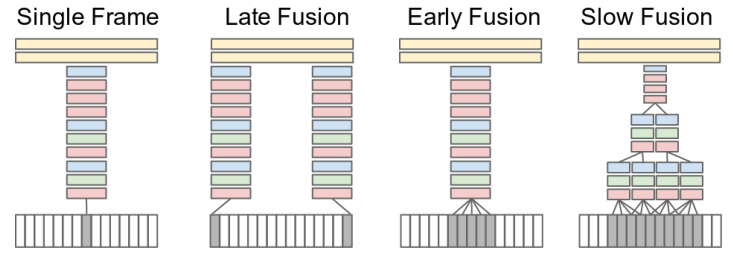
\includegraphics[scale=0.7]{fusions.PNG}
            \caption{Approaches for fusing information over temporal dimension}
            \label{fig:Figure 1}
        \end{figure}
    \end{enumerate}
    \item To speed up the network they combine two separate streams of processing. The context stream receives a down sampled version ($89\times 89$) of the original image ($178 \times 178$). The fovea stream receives the center $89\times 89$ region at the original resolution. This approach takes advantage of the camera bias present in many online videos, since object of interest often occupies the center region. This gives $2-4$ times speed up while maintaining the accuracy of the original network.
    \item They apply the prepossessing steps (crop and flips) consistently to all frames that are part of the same clip.
    \item The single frame detection actually performs ($60\% accuracy$) better that early and late fusion approach and only slightly worse than slow fusion ($60.9\%$). So they were not able to get much benefit from temporal connectivity. This was probably due to presence of camera motion in the video. Their model struggled to learn feature invariant to camera motion.
    \item They applied transfer learning on UCF-101 dataset which is much smaller. They tried three variants
    \begin{enumerate}
        \item Retraining only the softmax layer which does not perform best possibly because high level features are too specific to original dataset which only contains sports.
        \item Fine-tuning all layers also does not perform well possibly due to ovrefitting.
        \item Best performance is obtained by retraining only the top fully connected layers and freezing convolution layer weights.
    \end{enumerate}
    Training from scratch performs worse than transfer learning approach because of ovrefitting.
\end{itemize}

\end{document}
